\documentclass{article}
\usepackage[utf8]{inputenc}
\usepackage[margin=2cm]{geometry}
\usepackage{graphicx}
% \usepackage[numbers]{natbib}
\usepackage{amsmath}
\usepackage{amssymb}
\usepackage{mathtools}
% \usepackage{hyperref}
\usepackage{listings}
% \usepackage{xcolor}

\title{FYS-3033 Exam}
\author{Canditate}
\date{2022}
 
\begin{document}

\maketitle
\section{Assignment 1}
\subsection*{a)}
Cross entropy is a measurment of how diffrent two probability distributions are.
\begin{equation}
    \begin{split}
        H(z,y) &= -\sum_{i=0}^1 E_{yi}\log(z_i)\\
        &= -\left(1\cdot\log(z_0)+0\cdot\log(z_1)\right)\\
        &= -\log(z_0)\\    
    \end{split}
\end{equation}

\subsection*{b)}
If $\mathbf{z}$ are not stochastic then we cannot guarantee that the cross entropy function is defined. Any values of $z <= 0$ will not be defined by the cross entropy function. Even if we limit $z > 0$, the derivative of the cross entropy function approaches $0$ when $z$ gets large, which will inhibit learning.

\subsection*{c)}
\subsection*{d)}

\subsubsection*{Without regularization:}
\begin{equation}
    \begin{split} 
        \text{Because $y=(1,0)$ and the result in 1.a it follows that:}\\
        argmin_\mathbf{z} CE(\mathbf{z}; \mathbf{y})&=\begin{bmatrix}argmin_{z_0}(-log(z_0))\\1-argmin_{z_0}(-log(z_0))\end{bmatrix}\\
        &=\begin{bmatrix}1\\0\end{bmatrix} = \mathbf{y}
    \end{split}
\end{equation}

\subsubsection*{With $\ell^2$-regularization}
\begin{equation}
    \begin{split}
        argmin_\mathbf{z} CE(\mathbf{z}; \mathbf{y})+||\mathbf{z}||_2^2&=\begin{bmatrix}argmin_{z_0}(-log(z_0)+z_0^2+z_1^2)\\1-\left(argmin_{z_0}(-log(z_0)+z_0^2+z_1^2)\right)\end{bmatrix}\\
        solve(\frac{d}{dz_0}\left[-log(z_0)+z_0^2+z_1^2=0\right],z_0)&=argmin_{z_0}(-log(z_0)+z_0^2+z_1^2)\\
        \frac{d}{dz_0}\left[-log(z_0)+z_0^2+z_1^2\right]&=0\\
        \text{$z_1=1-z_0$}\\
        -\frac{1}{z_0}+2z_0-2(1-z_0)&=0\\
        4z_0^2-2z_0-1&=0, z_0\in(0,1)\\
        z_0 = \frac{1+\sqrt{5}}{4}\\
        argmin_\mathbf{z} CE(\mathbf{z}; \mathbf{y})+||\mathbf{z}||_2^2&=\begin{bmatrix}\frac{1+\sqrt{5}}{4}\\\frac{3-\sqrt{5}}{4}\end{bmatrix}\\
    \end{split}
\end{equation}

\subsubsection*{With $\ell^1$-regularization}
\begin{equation}
    \begin{split}
        argmin_\mathbf{z} CE(\mathbf{z}; \mathbf{y}) + ||\mathbf{z}||_1 &=\begin{bmatrix}argmin_{z_0}(-log(z_0)+ \sum_i |w_i|)\\1-\left(argmin_{z_0}(-log(z_0)+ \sum_i |w_i|)\right)\end{bmatrix}\\
        argmin_\mathbf{z} CE(\mathbf{z}; \mathbf{y}) + ||\mathbf{z}||_1 &=\begin{bmatrix}argmin_{z_0}(-log(z_0)+ |z_0|+|1-z_0|)\\1-\left(argmin_{z_0}(-log(z_0)+ |z_0|+|1-z_0|)\right)\end{bmatrix}\\
        z_0,z_1 \in (0,1)\Rightarrow\\
        argmin_\mathbf{z} CE(\mathbf{z}; \mathbf{y}) + ||\mathbf{z}||_1 &=\begin{bmatrix}argmin_{z_0}(-log(z_0)+ 1)\\1-\left(argmin_{z_0}(-log(z_0)+1)\right)\end{bmatrix}\\
        &=\begin{bmatrix}1\\0\end{bmatrix} = \mathbf{y}\\
    \end{split}
\end{equation}

\subsection*{e)}
The cross entropy function is at its minimum when $\mathbf{z}=\mathbf{y}$. If training is done using only cross entropy as a loss function, then ultimatly the predicted values of the training set will equall the trainingset labels. However, this will most likley mean that overfitting has taken place. By using $\ell^2$ regularization during training we ensure that the that we don't only try to replicate the training labels, but rather move towards them. On the other hand $\ell^1$ regularization can also result in predicted values becoming equall to the training labels, which again is a sure sign of overfitting.These results indicate that $\ell^2$ regularization works better to protect against overfitting, however $\ell^1$ regularization might be benefical to promote sparsity in the network if we have a large number of features. This is because $\ell^1$ regularization will make it beneficial for some values to be $0$. In 1.d the regularization paramater $\alpha$ is assumed to be one. However, if we include $\alpha$ in the regularization then $argmin_{z_0}(-log(z_0)+z_0^2+z_1^2)$ becomes: $$z_0=\frac{2\alpha + \sqrt{4\alpha^2+16\alpha}}{8\alpha}$$ If we let $\alpha\to\infty$ then $z_0\to\frac{1}{2}$, this shows that by having to high regularization paramater can harm performance.
\section{Assignment 2}
\subsection*{a)}
There are several methods that can be used to interpret a deep learning model. Class Model visualization and Class saliancy maps are to possible methods that can help interpret models. Class Model visualization tries to use a pretrained network and "train" an input to increase a specific class score. The technique works initiating a random input, feeding it through the network. Then calculating the gradient of the class score based on the input. Once this gradient is achieved then the input can be updated using gradient ascent. After repeating this process a certian number of times the final input should be an input that achieves high score for a specific class and can help a developer visualizing what the model is looking for on this specific class. Another similar technique is to choose a input from the test or training set, sending it through the model and again calculating the gradient of the class score with regards to the input. This gradient can be used to check what parts of the input affects the class score the most. Areas with high values in this gradient, should represent areas which when changed will affect the given class score the most. 
\subsection*{b)}
The VGG16 network is a deep convolutional network with relativley small receptive field. The argument behind this is that stacked receptive fields has collectively a larger receptive field.\cite[pp.2-3]{vgg16paper} In addition using stacked convolutional layer allows for several non-linear rectifying units. I implemented this using keras and tensorflow. After implementing a sequential model with all necassary layers, the image net weights from the original VGG16 where loaded into my model. Simonyan and Zisserman notes that adding $1x1$ convolutional layers to the network can be beneficial as it incorporates more non-linear rectifying units without affecting the receptive fields.\cite[pp.3]{vgg16paper}
\subsection*{c)}
The class model visualization for three diffrent classes are shown in figures \ref{fig::classModel2}-\ref{fig::classModel659}. The visualizations that were generated without gausian blur is predicted to be the class that we where after. For two of the visualizations generated using gausian blur the model predicts another class. However, for both of these the other class is a class that is very similar to the class we where after. This might be because the gausian filter removes some information that lives in the higher frequency of the image.
\begin{figure}[h]
    \begin{center}
        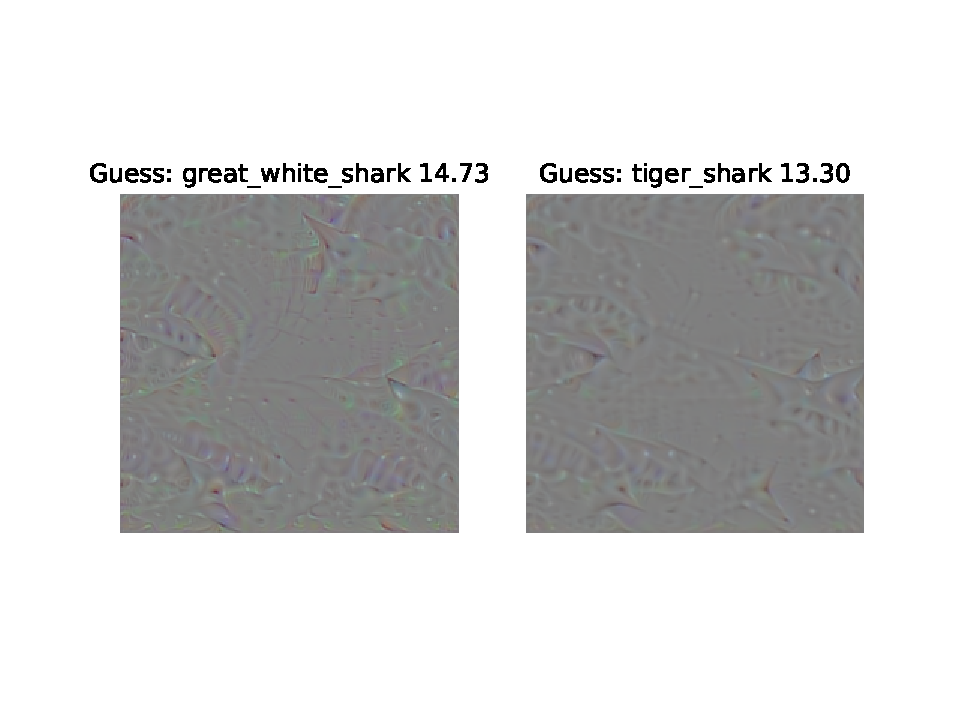
\includegraphics{../Task2/Figures/2_visualized.pdf}
        \caption{Class model visualization for the class white shark with its predicition and predicition score. [RIGHT] Class model visualization without gausian filtering [LEFT] Class model visualization with gausian filtering}
        \label{fig::classModel2}
    \end{center}
\end{figure}

\begin{figure}[h]
    \begin{center}
        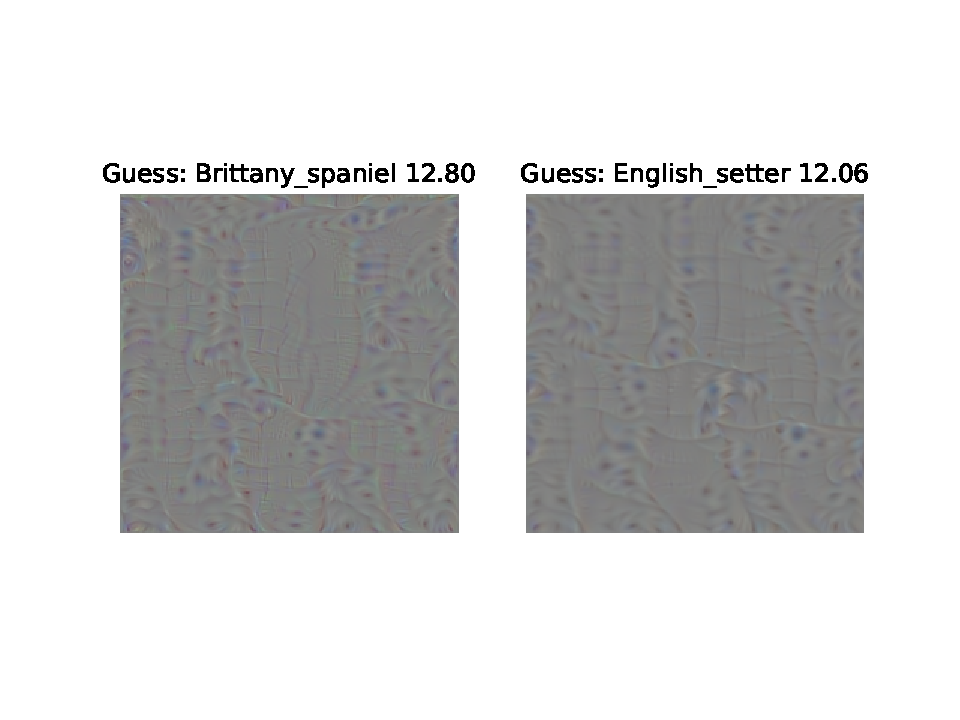
\includegraphics{../Task2/Figures/215_visualized.pdf}
        \caption{Class model visualization for the class brittany spaniel with its predicition and prediction score. [RIGHT] Class model visualization without gausian filtering [LEFT] Class model visualization with gausian filtering}
        \label{fig::classModel215}
    \end{center}
\end{figure}

\begin{figure}[h]
    \begin{center}
        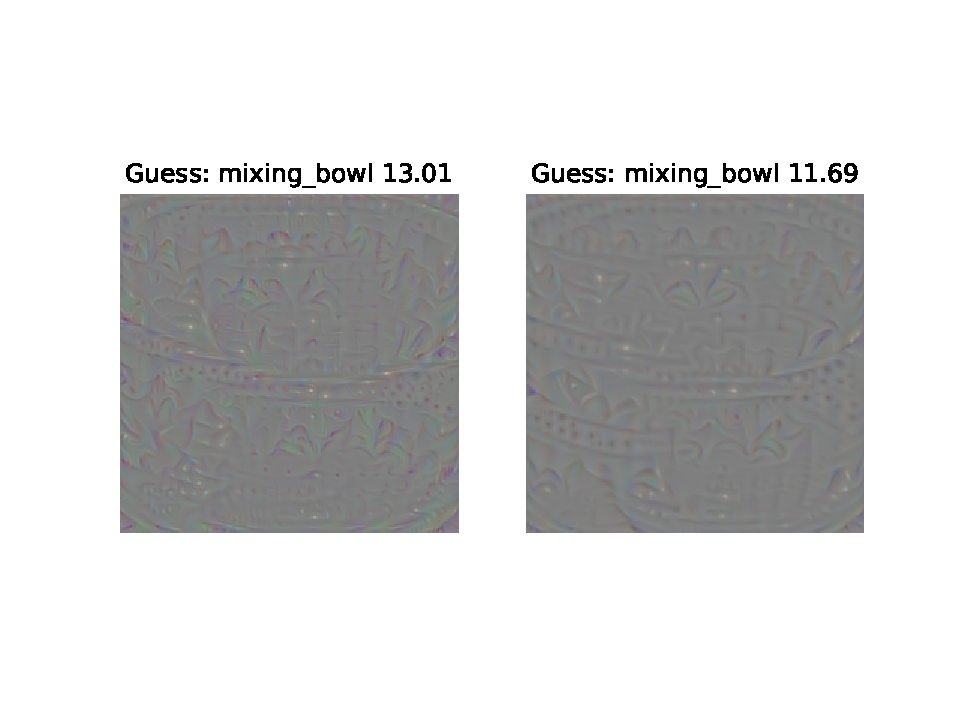
\includegraphics{../Task2/Figures/659_visualized.pdf}
        \caption{Class model visualization for the class mixing bowl with its predicition and prediction score. [RIGHT] Class model visualization without gausian filtering [LEFT] Class model visualization with gausian filtering}
        \label{fig::classModel659}
    \end{center}
\end{figure}

\subsection*{d)}
The top five predictions for the test images can be seen in figures \ref{fig::image1}-\ref{fig::image5}. For three of the images the top one prediction seem to be correct. For one the two that does not have a correct guess, a correct guess occurs in the top five predictions. Image number four has no correct guesses in the top five predictions, however, the confidence of the model is also quite week in this image.
\subsection*{e)}
The class saliancy maps for the top prediction of the test images can also be seen in figures \ref{fig::image1}-\ref{fig::image5}. The saliancy maps created without guided backpropogation are quite noicy but one can still see what parts of the images that affect the class score the most.
\subsection*{f)}
With saliancy maps computed using guided backpropogation the parts of the images that affects the class score most positivly are much clearer. We can see that for the wolf the most important part for the class score is the face of the wolf. With the eagle the most important part is the wings, even tough it classifies this image wrongly. It is interesting to note that the image of the two skiers much of the background also affect the class score. One can hypothezise that this is because skiing images often occur in snowy mountainous terrain, therefore the model will learn to associate this terrain with skiing.
\subsection*{g)}
Dropout is a technique often used in deep learning to prevent overfitting of data\cite{dropoutPaper}. The technique works by letting certian weights "drop" out of the network during training. This dropping out of nodes is done randomly based on some probability. The idea behind it is to allow nodes to learn to work for themselfs\cite{dropoutPaper}. Using dropout can also be seen as sampling results from a distribution of smaller networks. This can be used to model uncertaities. Normally when testing the network it is run with dropout turned of. By turning it on during inference and predicting on the same image several times one can take the mean of all predictions to find what prediction most subnetworks mostly agree upon. One can also calculate the variance over the predictions. Here a higher variance can be seen as higher disagreement between the subnetworks, and can therefore be seen as the uncertainty of the network.
\subsection*{h)}
The uncertainty and the predictive mean of the network for the test images can be seen in figures \ref{fig::image1}-\ref{fig::image5}. The uncertainty and predictive mean are calculated using 10 samples of subnetworks. For image 1 we can see that there is relativley high uncertainty regarding the predictions "ski" and "alps", this makes sense on the basis of the images nature. We can also se that the uncertainty for the wolf image is quite low in relation to the other images. For the image of the roof we can see that there is also relativly low uncertainty, however the confidence of the network is also low. This means that most subnetwork are also not very confident on their predictions.
\begin{figure}[h]
    \begin{center}
        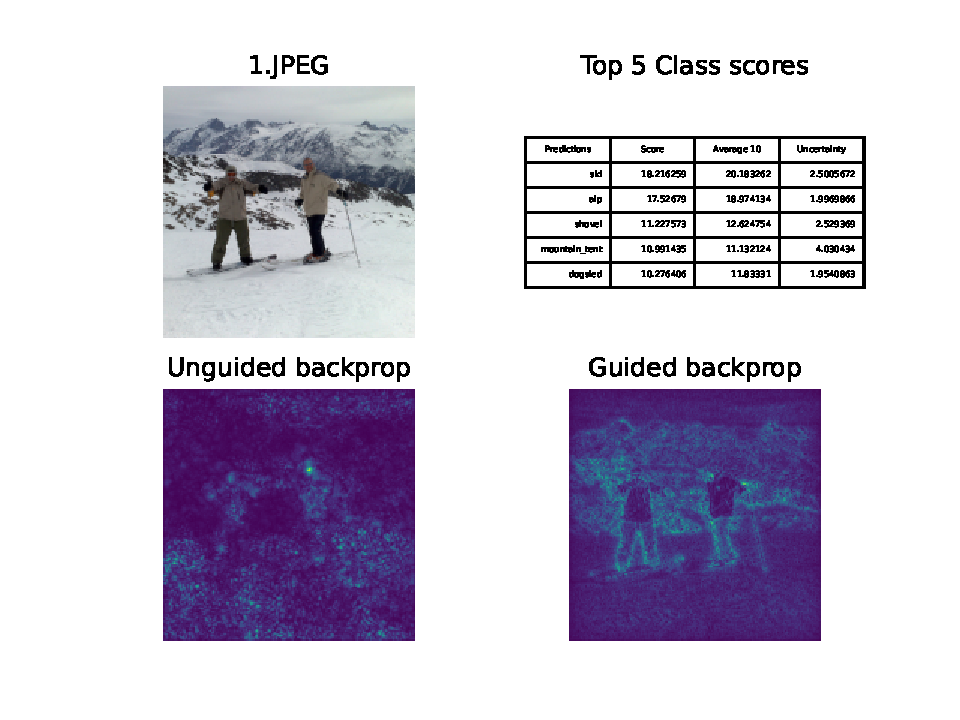
\includegraphics{../Task2/Figures/1.JPEG_k10_saliancy_uncertainty.pdf}
        \caption{Top five class scores of test image 1 with class saliancy map computed with and without guided backprop}
        \label{fig::image1}
    \end{center}
\end{figure}
\begin{figure}[h]
    \begin{center}
        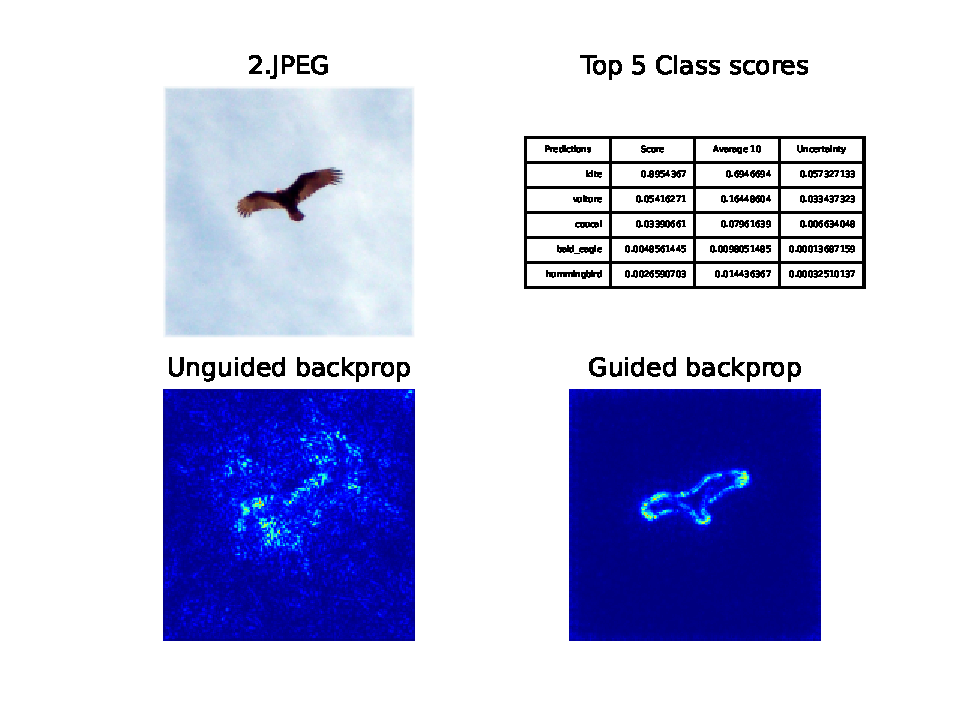
\includegraphics{../Task2/Figures/2.JPEG_k10_saliancy_uncertainty.pdf}
        \caption{Top five class scores of test image 2 with class saliancy map computed with and without guided backprop}
        \label{fig::image2}
    \end{center}
\end{figure}
\begin{figure}[h]
    \begin{center}
        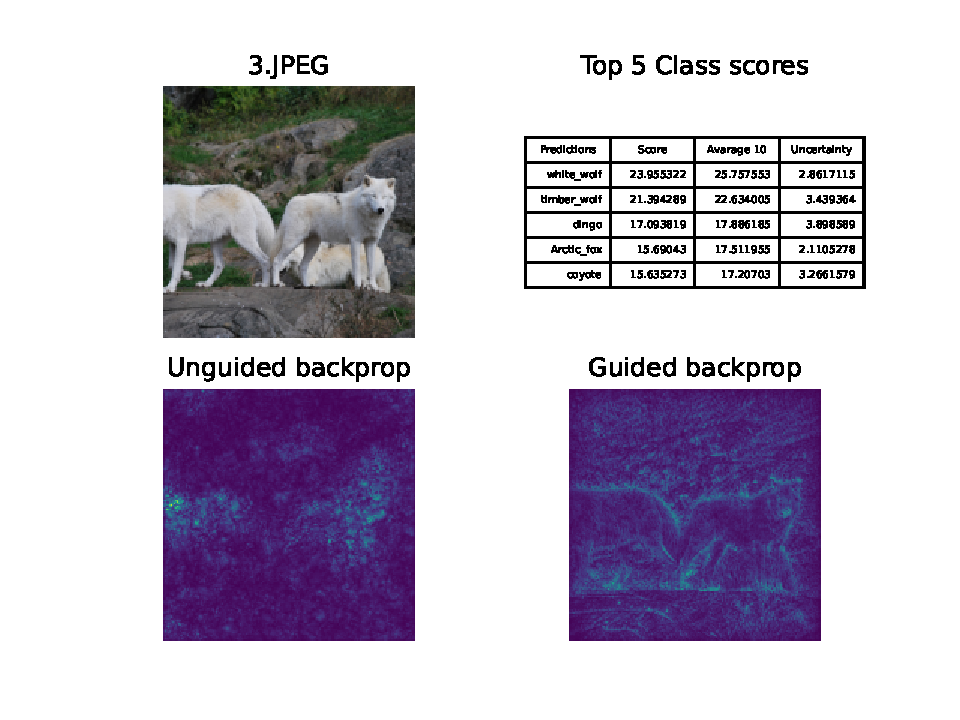
\includegraphics{../Task2/Figures/3.JPEG_k10_saliancy_uncertainty.pdf}
        \caption{Top five class scores of test image 3 with class saliancy map computed with and without guided backprop}
        \label{fig::image3}
    \end{center}
\end{figure}
\begin{figure}[h]
    \begin{center}
        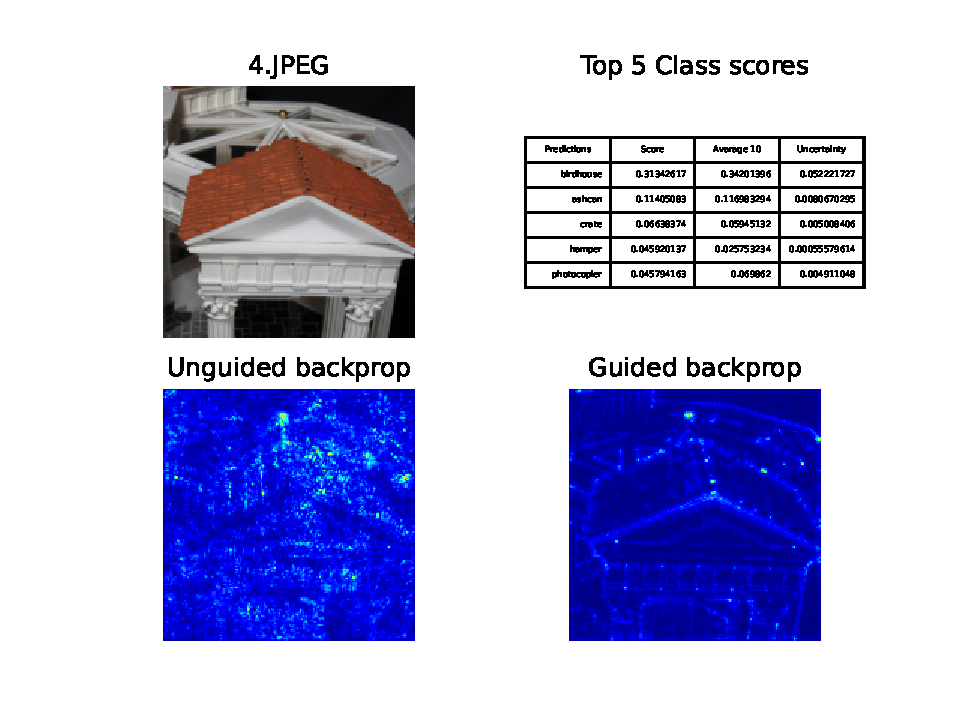
\includegraphics{../Task2/Figures/4.JPEG_k10_saliancy_uncertainty.pdf}
        \caption{Top five class scores of test image 4 with class saliancy map computed with and without guided backprop}
        \label{fig::image4}
    \end{center}
\end{figure}
\begin{figure}[h]
    \begin{center}
        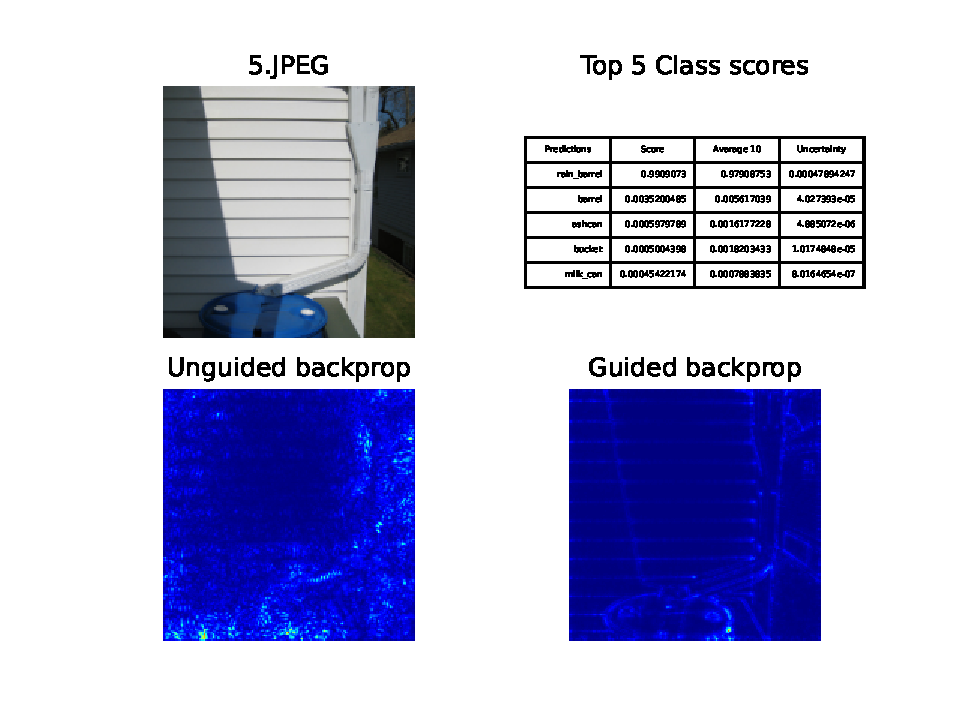
\includegraphics{../Task2/Figures/5.JPEG_k10_saliancy_uncertainty.pdf}
        \caption{Top five class scores of test image 5 with class saliancy map computed with and without guided backprop}
        \label{fig::image5}
    \end{center}
\end{figure}

\section{Assignment 3}
\subsection*{a)}
To design a network to deshuffle the images I started with the proposed VGG11 network. The result of training the VGG11 network for 100 epochs can be seen in figure \ref{fig::vgg11}. As expected this did not provide any good results. The next step was to apply batch normalization to the convolutional layers in the network. This allows the output of the convolutional layers to be normalized to a collective mean and standard deviation\cite{batchnorm}. The result of training the VGG11 network with batch normalization for 100 epochs can be seen in figure \ref{fig::vgg11bn}. This model worked alot better than the pure VGG11 network, however, it shows signs of extreme overfitting. To try to mitigate this $\ell^2$ regularization is applied to the classification part of the network. The result of training this new model for 100 epoch is shown in figure \ref{fig::vgg11bnl2}. The $\ell^2$ regularization clearly helped the overfitting of the network, however, it did not mitigate it completley. Rather it simply delayed the overfitting. In an atempt to further minimize the overfitting issue, dropout layers where added between the fully connected layers in the classification part. The result of this trainging can be seen in figure \ref{fig::vgg11bnl2do}
\begin{figure}[h]
    \begin{center}
        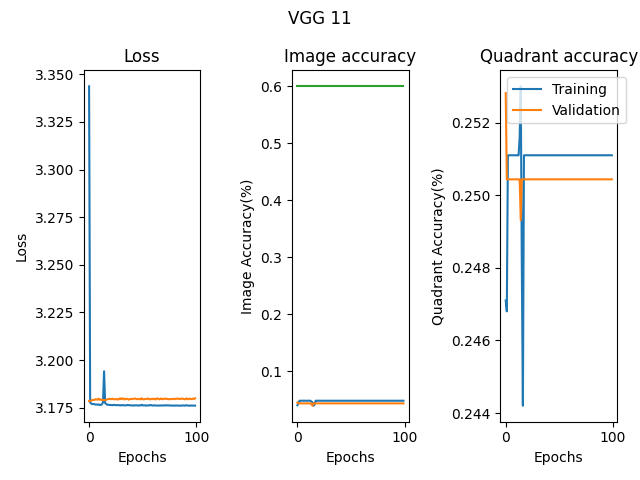
\includegraphics{../Task3/Figures/VGG11.png}
        \caption{Accuracy and loss of VGG11 network}
        \label{fig::vgg11}
    \end{center}
\end{figure}
\begin{figure}[h]
    \begin{center}
        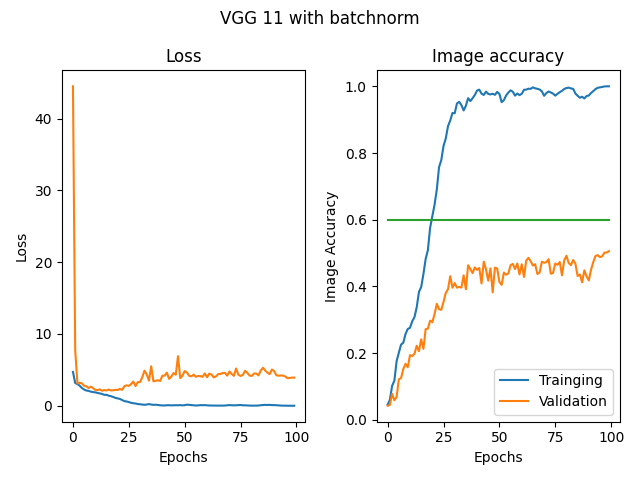
\includegraphics{../Task3/Figures/VGG11withbatchnorm.png}
        \caption{Accuracy and loss of VGG11 network with batch normalization on all convolutional layers}
        \label{fig::vgg11bn}
    \end{center}
\end{figure}
\begin{figure}[h]
    \begin{center}
        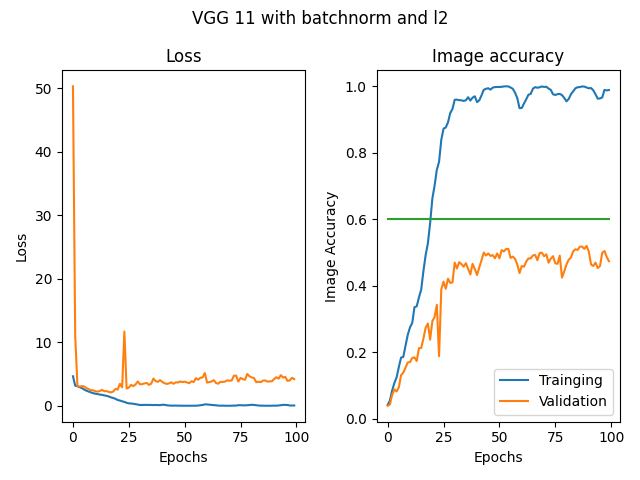
\includegraphics{../Task3/Figures/VGG11withbatchnormandl2.png}
        \caption{Accuracy and loss of VGG11 network with batch normalization on all convolutional layers and $\ell^2$ regularization on classification part of network.}
        \label{fig::vgg11bnl2}
    \end{center}
\end{figure}
\begin{figure}[h]
    \begin{center}
        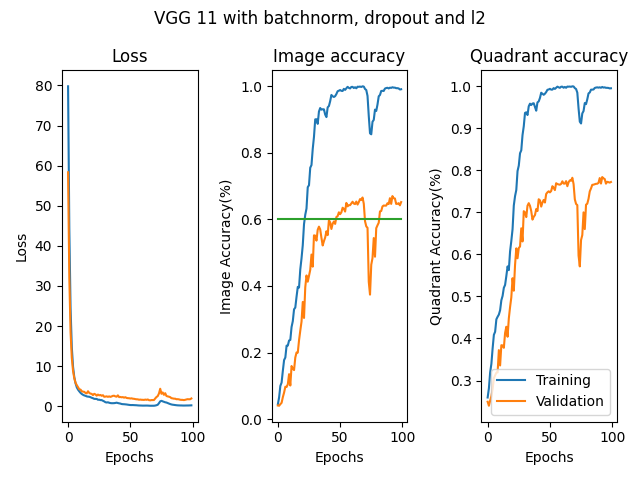
\includegraphics{../Task3/Figures/VGG11withbatchnorm,dropoutandl2.png}
        \caption{Accuracy and loss of VGG11 network with batch normalization on all convolutional layers and $\ell^2$ regularization on classification part of network.}
        \label{fig::vgg11bnl2do}
    \end{center}
\end{figure}
\subsection*{d)}

\bibliography{sources.bib}

\bibliographystyle{ieeetr}

\section{Appendix} 
\subsection{Task 2:}
\lstinputlisting[language=Python]{../Task2/task2.py}
\subsection{Task 3:}
\lstinputlisting[language=Python]{../Task3/permutation.py}
\lstinputlisting[language=Python]{../Task3/task3.py}

\end{document}
